\documentclass{article}
\usepackage{graphicx}
\usepackage{amsmath}
% avoid new line with a tab
\usepackage[parfill]{parskip}
\usepackage{hyperref}
\graphicspath{ {./figures/} }

\title{COMP.SEC.220 Security Protocol\footnote{github - \url{https://github.com/ancuongnguyen07/SecurityProtocol}}}
\author{Cuong Nguyen - LAB 1}
\date{22/04/2022}

\begin{document}
    
\maketitle

\section*{Exercise 1}
%
\begin{figure}[hpt]
    \centering
    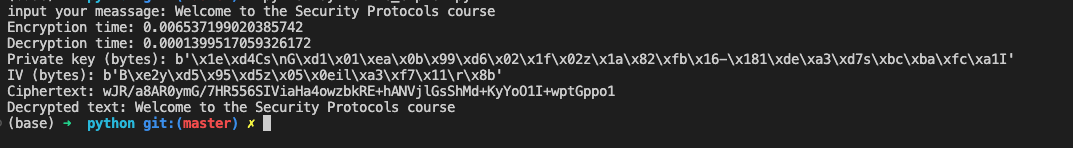
\includegraphics[width=100mm, height=80mm]{aes.png}
    \caption{AES-256-CBC-mode encrytion-decrytion time}
    \label{fig:aes-cbc}
\end{figure}

% \section*{Exer}

\end{document}